\documentclass[a4paper,12pt]{extreport}
\usepackage[utf8]{inputenc}
\usepackage[russian]{babel}
\usepackage{ragged2e}
\usepackage[mag=1000,a4paper,left=1cm,right=1cm,top=1cm,bottom=1cm,noheadfoot]{geometry}
\usepackage{mathtext}
\usepackage{amsmath,amssymb,amsthm,amscd,amsfonts,graphicx,epsfig,textcomp,wrapfig}
\usepackage[dvips]{graphicx}
\graphicspath{{noiseimages/}}

\newcommand{\tab}{\hspace{10mm}}
\newcommand{\name}{
			\normalsize
			{
				\ \ \quad
                \mbox{} \hfil {\flushleft{5 лицей}} \hfill {12.10.2023}
			%\quad
			}
			\vspace{5pt}\hrule
		}

\def\head#1#2{
	\begin{center}{
			\LARGE
			\bf #2
			
			{\normalsize \bf #1}
			\vspace{-10pt}
	}\end{center}
}

\newcommand{\del}{\mathop{\raisebox{-2pt}{\vdots}}}
\newcommand{\q}{}

\newcounter{tasknum}
\setcounter{tasknum}{0}
\def\thetasknum{{\textbf{\arabic{tasknum}}}}
\newcommand{\task}{\refstepcounter{tasknum}\vspace{2pt}\noindent \textbf{} \thetasknum\textbf{.}~}
\newcommand{\coff}{\refstepcounter{tasknum}\vspace{2pt}\noindent \textbf{Задача} \thetasknum *\textbf{.}~}


\newcommand{\eq}[1]{\underset{#1}{\equiv}}
\newcommand{\dv}{\ensuremath{\mathop{\raisebox{-2pt}{\vdots}}}}
\newcommand{\ndv}{\not \dv}

\newcounter{exnum}
\setcounter{exnum}{0}
\def\theexnum{{\emph{\arabic{exnum}}}}
\newcommand{\ex}{\refstepcounter{exnum}\vspace{2pt}\noindent \emph{Упражнение} \theexnum\emph{.}~}



\theoremstyle{plain}
\newtheorem{theorem}{Теорема}
\newtheorem{lemma}{Лемма}
\newtheorem{proposition}{Предложение}
\newtheorem{corollary}{Следствие}
\theoremstyle{definition}
\newtheorem{definition}{Определение}
\theoremstyle{remark}
\newtheorem{remark}{Замечание}
\newtheorem{example}{Пример}

\textheight=250mm %
\textwidth=180mm %
\oddsidemargin=-10.4mm%
\evensidemargin=-10.4mm %
\topmargin=-24.4mm


\begin{document}
	\pagestyle{empty}
    \name{}
	\head{6 класс}{Игры позиции}
	\bigskip
	
\task На доске $11 \times 15$ в левом нижнем углу стоит хромой конь. Двое ходят по очереди. За ход разрешается передвигать коня на две клетки вправо и одну клетку вверх или на две клетки вверх и на одну вправо. Кто не может сделать ход — проиграл.\\

\task В левом нижнем углу доски $6 \times 6$ стоит фишка. За один ход можно подвинуть фишку или на одну клетку вверх, или на две клетки вправо или на одну клетку вправо и одну клетку вверх. Проигрывает тот, кто не может сделать ход. Кто выигрывает при правильной игре?\\

\task На картинке слева в вершине под номером $1$ стоит фишка. Два игрока по очереди двигают её по стрелкам. Игра заканчивается, когда ходить больше нельзя. При этом тот, кто привёл фишку в вершину $12$, проигрывает, а тот, кто привёл в $11$ или $13$ – выигрывает. Кто выигрывает при правильной игре, начинающий или его соперник?\\

\begin{figure}[h]
\centering
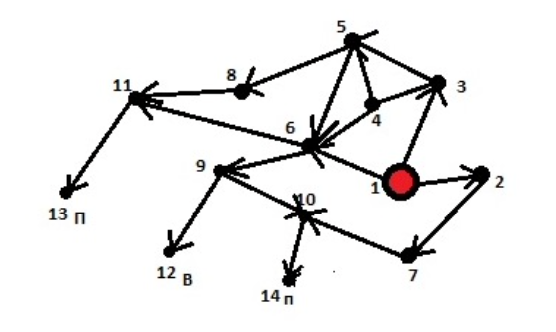
\includegraphics[width=0.35\linewidth]{game.png}
\label{fig:mpr}
\end{figure}

\task Двое игроков ходят по очереди на циферблате с одной стрелкой: каждый своим ходом переводит стрелку на два или три часа вперед. В начале игры стрелка показывает полдень. Выигрывает тот, кто первым поставит стрелку на $11$ часов. (Стрелка может сделать несколько оборотов, прежде чем указать на $11$ часов.)\\

\task На доске $16 \times 16$ стоит ферзь. Его можно двигать либо вверх, либо вправо, либо вправо-вверх. Проигрывает тот, кто не может ходить. При каких начальных положениях ферзя второй игрок победит?\\

\task Игра начинается с числа $4$. За ход разрешается прибавить к имеющемуся числу любое меньшее натуральное число. Выигрывает тот, кто получит $2023$.\\

\task Однажды на волшебном дереве выросло 300 золотых монет. Кот Базилио и лиса Алиса договорились по очереди каждую ночь ходить к этому дереву и забирать не более половины имеющихся на нём монет. Если кто-то из них не может больше сорвать ни одной монеты, то отдает другому всё, что успел взять. Первой пошла Алиса. Кто останется в дураках?\\

\task В двух кучах $n$ и $k$ камней соответственно. За один ход можно либо взять несколько камней из одной кучи, либо поровну из двух куч. Проигрывает тот, кто не может сделать ход. Для каких $n$ и $k$, не превосходящих $15$, у начинающего игрока нет выигрышной стратегии?\\


\end{document}
